\documentclass[12pt]{beamer}
\usetheme{Penn} 
\usepackage{amsmath, amssymb, amsthm, amsfonts}
\usepackage{graphicx}
\usepackage{fancyvrb}
\usepackage{verbatim}
%\usepackage{tabularx}
\usepackage{tikz}
\usepackage{animate}
\usetikzlibrary{matrix, shapes, arrows, calc, backgrounds}
\usepackage[vcentermath, enableskew]{youngtab}
\newcommand{\ZZ}{\ensuremath{\mathbb{Z}}}
\newcommand{\RR}{\ensuremath{\mathbb{R}}}
\newcommand{\PP}{\ensuremath{\mathbb{P}}}

\newcommand{\CC}{\ensuremath{\mathbb{C}}}

\newtheorem{thm}{Theorem}[section]
\newtheorem{cor}[thm]{Corollary}
\newtheorem{lem}[thm]{Lemma}
\newtheorem{prop}[thm]{Proposition}
\theoremstyle{definition}
\newtheorem{conj}[thm]{Conjecture}
\newtheorem{defn}[thm]{Definition}
\newtheorem{ex}[thm]{Example}
\newtheorem{rmk}[thm]{Remark}
\newtheorem{alg}[thm]{Algorithm}
\newtheorem{question}[thm]{Question}
\begin{document}

\author[Z. Rosen]{Zvi Rosen \\ Department of Mathematics}

\date[\today]{\today}
\title[Cholesky Factorization]{{\Large Cholesky Factorization}}
\institute[Dept. of Mathematics~~--~~University of Pennsylvania]{}


\frame{\titlepage}


\begin{frame}
\frametitle{LU Factorization}
Any matrix $A$, after permuting the rows of $A$ with a permutation 
matrix $P$,
can be factorized as $PA = LU$ where:\\ \vspace{4mm}
$L$ is lower-triangular, and\\
$U$ is upper-triangular. \\ \vspace{4mm}

The MATLAB command {\tt [L,U,P] = lu(A)} obtains the LU Factorization.

\end{frame}


\begin{frame}
\frametitle{LU Factorization - Example}
We define the following matrix:

\[
A = \left[ \begin{array}{ccc} 
7.102 & 3.431 & 5.528 \\
    8.412 & 2.135 & 1.709 \\
    4.047 & 5.210 & 8.227 \\
\end{array} \right]
\]

The command {\tt [L,U] = lu(A)} gives an upper-triangular
and ``lower-triangular'' matrix whose product is $A$. \\ \vspace{4mm}

Changing the pivot options can sometimes give an ``honest''
lower-triangular matrix.

\end{frame}

\begin{frame}
\frametitle{LU for Symmetric Matrices}

Recall: A symmetric matrix $A$ is a matrix whose entries
$a_{ij} = a_{ji}$ for all $i,j$. Equivalently, $A = A^T$.

The LU factorization for $A$ can be $A = U^TU$. I.e. the
lower-triangular matrix is the transpose of the upper-triangular
matrix. This factorization is called the {\em Cholesky factorization}.

\end{frame} 

\begin{frame}
\frametitle{Andre-Louis Cholesky}
\centerline{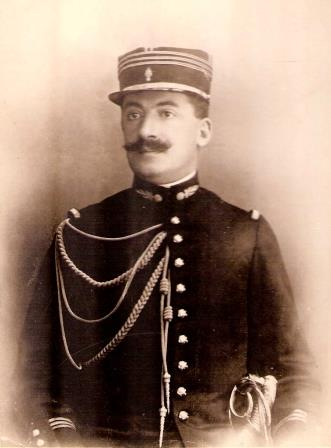
\includegraphics{cholesky.jpg}}
\end{frame}

\begin{frame}
\frametitle{Cholesky factorization - example}

\[
A = \left[ \begin{array}{ccc} 
7.102 & 3.431 & 5.528 \\
     3.431 & 2.135 & 1.709 \\
    5.528 &  1.709 & 8.227 \\
\end{array} \right] \] \[ =
\left[ \begin{array}{ccc} 
u_{11} & 0 & 0 \\
u_{21} & u_{22} & 0 \\
u_{31}  & u_{32} & u_{33}\\
\end{array} \right]
\left[ \begin{array}{ccc} 
u_{11} & u_{21} &  u_{31} \\
0 & u_{22} &  u_{32} \\
0 & 0  & u_{33}\\
\end{array} \right] \]
Note that $a_{11} = u_{11}^2$, so set $u_{11} = \sqrt{7.102}$. \\
Moving to the next row, $u_{21}u_{11} = a_{21}$ so set $u_{21} = 3.431/7.102 = .4831$.\\
We know $a_{22} = u_{21}^2 + u_{22}^2$ so solve: $u_{22} = \sqrt{a_{22} - u_{21}^2} = \sqrt{2.135 - .4831^2} = 1.379$. Etc.
\end{frame} 

\begin{frame}
\frametitle{General formula for Cholesky Entries}

The general formula for diagonal entries is:
\[ u_{ii} = \sqrt{a_{ii} - \sum_{k =1}^{i-1} u_{ki}^2}. \]
The general formula for off-diagonal entries is:
\[ u_{ij} = \dfrac{a_{ij} - \sum_{k=1}^{i-1} u_{ki}u_{kj}}{u_{ii}}\]
\end{frame}

\begin{frame}
\frametitle{Cholesky in MATLAB}

In MATLAB, the Cholesky decomposition of a matrix $A$ is obtained
using the command {\tt U =  chol(A)}.
\end{frame}
\end{document}
